\documentclass{article}

  \usepackage{import}
  \usepackage{defaultHeader}

\begin{document}
\title{Math Handbook}
\author{Cody Barnson}
\date{\today}
\pagenumbering{gobble}
\maketitle
\tableofcontents

% macro inserts list of all floated listings
\renewcommand\listoflistingscaption{Code segments}
% \listoflistingscaption

% call after redefining listoflistingscaption
% \listoflistings

% changes the caption on all the listings tables
% e.g. "Code snippet 1: Example"
\renewcommand\listingscaption{Code snippet}
% \listingscaption

% \newpage
\pagenumbering{arabic}
% \listoftables
% \listoffigures
% \newpage

% TIPS
% modulus: \bmod{k} or \pmod{k}
% logical and/or: \land \lor

% ----------------------------------------
% BEGIN
% ----------------------------------------

% Full sized fractions, even inline, use \dfrac{}{}
% \( \dfrac{\sqrt 2}{2} \bigg/ \frac{\sqrt 2}{2} \bigg/ \tfrac{\sqrt 2}{2} \)

\section{Math}

\subsubsection{Limits}
\begin{equation}
    \lim_{a\to \infty} \tfrac{1}{a}
\end{equation}


\begin{equation}
    \lim\nolimits_{a\to \infty} \tfrac{1}{a}
\end{equation}

\subsubsection{Log base conversion}
\begin{equation*}
    \frac{log_xn}{log_xB} = log_Bn
\end{equation*}

\subsubsection{Ceiling integer division}
\begin{align*}
    \left\lfloor\dfrac{n}{d}\right\rfloor & = \frac{n + d - 1}{d} \\
\end{align*}

\subsubsection{Bit shift equivalent of multiply by 10}
\begin{minted}[frame=lines,framesep=2mm,fontsize=\footnotesize,bgcolor=LightGray,tabsize=4,numbersep=4pt,resetmargins,samepage,mathescape,linenos,gobble=2]{cpp}
    // $(x << 3) + (x << 1) \equiv x * 10$
    int x, y;
    // ...
    x = (x << 3) + (x << 1);
    y = y * 10;
    assert(x == y);
\end{minted}

\noindent\rule{\textwidth}{1pt}

\section{Programming}
\subsection{C++}
\subsubsection{Logarithm base 2}

\begin{minted}[frame=lines,framesep=2mm,fontsize=\footnotesize,bgcolor=LightGray,tabsize=4,numbersep=4pt,resetmargins,samepage,mathescape,linenos,gobble=2]{cpp}
    // $log_2(n)$
    log2(n) = 31 - __builtin_clz(n);
\end{minted}


\subsubsection{Add value, update average}
\begin{minted}[frame=lines,framesep=2mm,fontsize=\footnotesize,bgcolor=LightGray,tabsize=4,numbersep=4pt,resetmargins,samepage,mathescape,linenos,gobble=2]{cpp}
    // $avg_{n+1} = \dfrac{sum_n(n+1) + kn - sum}{n(n + 1)}$
    int n, sum;
    // ...
    double avg = sum / n;
    while ((int)(avg + 0.5) < k) {
        avg = sum * n + sum + k * n - sum;
        avg /= n * n + n;
        sum += k;
        n++;
    }
\end{minted}

\subsubsection{Binomial coefficient}
\begin{minted}[frame=lines,framesep=2mm,fontsize=\footnotesize,bgcolor=LightGray,tabsize=4,numbersep=4pt,resetmargins,samepage,mathescape,linenos,gobble=2]{cpp}
    // ${n\choose k} = {n-1\choose k-1} + {n-1\choose k}$
    typedef long long ll;
    ll binom(int n, int k) {
        if (k == 0 || k == n) return 1;
        k = min(k, n - k); // Since ${n\choose k} \equiv {n\choose n-k}$
        ll ans = 1LL;
        for (ll i = 1; i <= k; i++) {
            ans = ans * (n - k + i) / i;
        }
    }
    ll choose(int n, int k, ll p = 1e9+7) {
        if (n < k) return 0;
        k = min(k, n - k);
        ll num = 1, den = 1;
        for (int i = 0; i < k; i++) num = num * (n - i) % p;
        for (int i = 1; i <= k; i++) den = den * i % p;
        return num * powmod(den, p - 2, p) % p;
    }
    ll multichoose(int n, int k, ll p = 1e9+7) {
        return choose(n + k - 1, k, p);
    }
\end{minted}

\subsubsection{Catalan numbers}
\begin{minted}[frame=lines,framesep=2mm,fontsize=\footnotesize,bgcolor=LightGray,tabsize=4,numbersep=4pt,resetmargins,samepage,mathescape,linenos,gobble=2]{cpp}
    typedef long long ll;
    ll catalan(int n, ll p = 1e9+7) {
        return choose(2 * n, n, p) * powmod(n + 1, p - 2, p) % p;
    }
    ll powmod(ll x, ll n, ll m) {
        ll a = 1, b = x;
        for (; n > 0; n >>= 1) {
            if (n & 1) a = mulmod(a, b, m);
            b = mulmod(b, b, m);
        }
        return a % m;
    }
    ll mulmod(ll x, ll n, ll m) {
        ll n = 0, b = x % m;
        for (; n > 0; n >>= 1) {
            if (n & 1) a = (a + b) % m;
            b = (b << 1) % m;
        }
        return a % m;
    }
\end{minted}

\subsubsection{Count number of digits in a number}
\begin{minted}[frame=lines,framesep=2mm,fontsize=\footnotesize,bgcolor=LightGray,tabsize=4,numbersep=4pt,resetmargins,samepage,mathescape,linenos,gobble=2]{cpp}
    // digits = $\floor{log_{10}(n)} + 1$
    int countDigits(long long n) {
        return n > 0 ? (int)log10((double)n) + 1 : 1;
    }
\end{minted}

\subsubsection{Enumerate combinations of N elements in K in lexical order}
\begin{minted}[frame=lines,framesep=2mm,fontsize=\footnotesize,bgcolor=LightGray,tabsize=4,numbersep=4pt,resetmargins,samepage,mathescape,linenos,gobble=2]{cpp}
    // $N, K \in  \mathbb{N}$, consider set numbers $1 \dots N$, derive all its different subsets of 
    // cardinality $K$, in lexical order.
    bool next_combination(vector<int> &a, int n) {
        int k = a.size();
        for (int i = k - 1; i >= 0; --i) {
            if (a[i] < n - k + i + 1) {
                ++a[i];
                for (int j = i + 1; j < k; ++j) {
                    a[j] = a[j - 1] + 1;
                }
                return true;
            }
        }
        return false;
    }
\end{minted}

\subsubsection{Prime factorization}
\begin{minted}[frame=lines,framesep=2mm,fontsize=\footnotesize,bgcolor=LightGray,tabsize=4,numbersep=4pt,resetmargins,samepage,mathescape,linenos,gobble=2]{cpp}
    typedef vector<int> vi;
    vi factor(int n) {
        vi f;
        if (n < 2) return vi();
        while (~n & 1) n /= 2, f.push_back(2);
        for (long long p = 3; p * p <= n; p += 2) 
            while (n % p == 0) n /= p, f.push_back((int)p);
        if (n > 1) f.push_back(n);
        return f;
    }
\end{minted}

\subsubsection{Fibonacci}
\begin{minted}[frame=lines,framesep=2mm,fontsize=\footnotesize,bgcolor=LightGray,tabsize=4,numbersep=4pt,resetmargins,samepage,mathescape,linenos,gobble=2]{cpp}
    // Matrix Exponentiation method
    // Complexity: $O(log(n))$
    // $fib(0) = 0, fib(1) = 1$
    // Note: $fib(\ge 47)$ will overflow a 32-bit signed integer
    int f[1000];
    int fib(int n) {
      if (n < 2) return n;
      if (f[n]) return f[n];
      int k = (n + 1) / 2;
      f[n] = (n & 1) ? fib(k) * fib(k) + fib(k - 1) * fib(k - 1)
                     : (2 * fib(k - 1) + fib(k)) * fib(k);
      return f[n];
    }
\end{minted}

\subsubsection{Modular Exponentiation}
\begin{minted}[frame=lines,framesep=2mm,fontsize=\footnotesize,bgcolor=LightGray,tabsize=4,numbersep=4pt,resetmargins,samepage,mathescape,linenos,gobble=2]{cpp}
    // Complexity: $O(log(n))$
    // Compute $x^n mod m$
    int modexp(int x, int n, int m) {
      if (n == 0) return 1;
      if (n & 1) return ((x % m) * modexp(x, n - 1, m)) % m;
      int y = modexp(x, n / 2, m);
      return (y * y) % m;
    }
\end{minted}

\subsubsection{Sieve + Optimized primality testing}
\begin{minted}[frame=lines,framesep=2mm,fontsize=\footnotesize,bgcolor=LightGray,tabsize=4,numbersep=4pt,resetmargins,samepage,mathescape,linenos,gobble=2]{cpp}
    // Sieve + optimized prime testing
    typedef long long ll;
    typedef vector<int> vi;

    ll sz;
    bitset<10000010> p; // $10^7+10$
    vi primes;
    void sieve(ll m) {
        sz = m + 1;
        p.set();
        p[0] = p[1] = 0;
        for (ll i = 2; i <= sz; i++) {
            if (p[i]) {
                for (ll j = i * i; j <= sz; j += i) {
                    p[j] = 0;
                }
                primes.push_back((int)i);
            }
        }
    }
    bool isPrime(ll x) {
        if (x <= sz) return p[x];
        for (int i = 0; i < (int)primes.size(); i++) {
            if (x % primes[i] == 0) return false;
        }
        return true;
    }
\end{minted}

\subsubsection{Base conversion}
\begin{minted}[frame=lines,framesep=2mm,fontsize=\footnotesize,bgcolor=LightGray,tabsize=4,numbersep=4pt,resetmargins,samepage,mathescape,linenos,gobble=2]{cpp}
    // Base conversion
    // Complexity: $O(N)$, N digits
    // Given digits of int x in base a, return x's digits in base b.
    
    typedef vector<int> vi;

    // x : digit representation of number
    // a : base of x
    // b : desired base
    // returns => vector<int> digits of number in base b.
    // Note: vec[0] stores the most significant digit.
    vi convert_base(const vi &x, int a, int b) {
        unsigned long long base10 = 0;
        FR(i, x.size()) base10 += x[i] * pow(a, x.size() - i - 1);
        int N = ceil(log(base10 + 1) / log(b));
        vi bb;
        for (int i = 1; i <= N; i++)
            bb.emplace_back((int)(base10 / pow(b, N - i)) % b);
        return bb;
    }

    // x : number
    // b : desired base
    // returns => vector<int> digits of number in base b
    vi base_digits(int x, int b = 10) {
        vi bb;
        while (x != 0) bb.emplace_back(x % b), x /= b;
        reverse(begin(bb), end(bb));
        return bb;
    }

    int main() {
        // consider $123_5$, (i.e. $123$ in base $5$)
        vi x{1, 2, 3}; int a = 5;
        vi z = convert_base(x, a, 10); // $123_5 = 38_{10}$, z = {3, 8}
        vi y = convert_base(x, a, 3); // $123_5 = 1102_{3}$, y = {1, 1, 0, 2}
    }
\end{minted}

\section{\LaTeX}

\subsection{Learning Resources}
\begin{itemize}
    \item \href{https://en.wikibooks.org/wiki/LaTeX}{LaTeX Wiki}
    \item \href{http://detexify.kirelabs.org/classify.html}{Detexify}
    \item \href{Uhttps://www.ctan.org/tex-archive/info/symbols/comprehensiveRL}{The Comprehensive LaTeX Symbol List}
    \item \href{http://mathlex.org/latex}{LaTeX Utility}
    \item \href{https://www.maths.tcd.ie/~dwilkins/LaTeXPrimer/}{LaTeX Primer}
    \item \href{https://www.tug.org/utilities/plain/cseq.html}{TeX Primitive Control Sequences}
    \item \href{http://www-h.eng.cam.ac.uk/help/tpl/textprocessing/}{Cambridge Text Processing using LaTeX}
\end{itemize}

% \subsection{}
% TODO: \href{}{}

\subsection{Picture}

For more information, see \href{https://en.wikibooks.org/wiki/LaTeX/Picture}{Picture}.  Also, see \href{https://en.wikipedia.org/wiki/Gnuplot}{Gnuplot}.

\paragraph{Draw arrows}
\begin{Verbatim}[fontsize=\scriptsize]
    \setlength{\unitlength}{0.75mm}
    \begin{picture}(60,40)
        \put(30,20){\vector(1,0){30}}
        \put(30,20){\vector(4,1){20}}
        \put(30,20){\vector(3,1){25}}
        \put(30,20){\vector(2,1){30}}
        \put(30,20){\vector(1,2){10}}
        \thicklines
        \put(30,20){\vector(-4,1){30}}
        \put(30,20){\vector(-1,4){5}}
        \thinlines
        \put(30,20){\vector(-1,-1){5}}
        \put(30,20){\vector(-1,-4){5}}
    \end{picture}
\end{Verbatim}
\setlength{\unitlength}{0.75mm}
\begin{picture}(60,40)
    \put(30,20){\vector(1,0){30}}
    \put(30,20){\vector(4,1){20}}
    \put(30,20){\vector(3,1){25}}
    \put(30,20){\vector(2,1){30}}
    \put(30,20){\vector(1,2){10}}
    \thicklines
    \put(30,20){\vector(-4,1){30}}
    \put(30,20){\vector(-1,4){5}}
    \thinlines
    \put(30,20){\vector(-1,-1){5}}
    \put(30,20){\vector(-1,-4){5}}
\end{picture}

\paragraph{Text and formulae with \texttt{put} command}
\begin{Verbatim}[fontsize=\scriptsize]
    \setlength{\unitlength}{0.8cm}
    \begin{picture}(6,5)
        \thicklines
        \put(1,0.5){\line(2,1){3}}
        \put(4,2){\line(-2,1){2}}
        \put(2,3){\line(-2,-5){1}}
        \put(0.7,0.3){$A$}
        \put(4.05,1.9){$B$}
        \put(1.7,2.95){$C$}
        \put(3.1,2.5){$a$}
        \put(1.3,1.7){$b$}
        \put(2.5,1.05){$c$}
        \put(0.3,4){$F=\sqrt{s(s-a)(s-b)(s-c)}$}
        \put(3.5,0.4){$\displaystyle s:=\frac{a+b+c}{2}$}
    \end{picture}
\end{Verbatim}
\setlength{\unitlength}{0.8cm}
\begin{picture}(6,5)
    \thicklines
    \put(1,0.5){\line(2,1){3}}
    \put(4,2){\line(-2,1){2}}
    \put(2,3){\line(-2,-5){1}}
    \put(0.7,0.3){$A$}
    \put(4.05,1.9){$B$}
    \put(1.7,2.95){$C$}
    \put(3.1,2.5){$a$}
    \put(1.3,1.7){$b$}
    \put(2.5,1.05){$c$}
    \put(0.3,4){$F=\sqrt{s(s-a)(s-b)(s-c)}$}
    \put(3.5,0.4){$\displaystyle s:=\frac{a+b+c}{2}$}
\end{picture}


\subsection{Mathematics}
TODO: \href{https://en.wikibooks.org/wiki/LaTeX/Mathematics}{Mathematics}

\subsection{Document Structure}
TODO: \href{https://en.wikibooks.org/wiki/LaTeX/Document_Structure}{Document Structure}

\subsection{Footnotes and Margin Notes}
TODO: \href{https://en.wikibooks.org/wiki/LaTeX/Footnotes_and_Margin_Notes}{Footnotes and Margin Notes}

\subsubsection{Creating a footnote}
This is a footnote.\footnote{And here is the footnote text.}

\subsection{Package Reference}
TODO: \href{https://en.wikibooks.org/wiki/LaTeX/Package_Reference}{Package Reference}

\subsection{Font}
\subsubsection{Font sizes}
\begin{table}[H]
    \centering
    \begin{tabular}[]{lr}
        \Huge{texblog.org}         & \verb|\Huge|  \\
        \huge{texblog.org}         & \verb|\huge|  \\
        \LARGE{texblog.org}        & \verb|\LARGE|  \\
        \Large{texblog.org}        & \verb|\Large|  \\
        \large{texblog.org}        & \verb|\large|  \\
        \normalsize  {texblog.org} & \verb|\normalsize  |  \\
        \small{texblog.org}        & \verb|\small|  \\
        \footnotesize{texblog.org} & \verb|\footnotesize|  \\
        \scriptsize{texblog.org}   & \verb|\scriptsize| \\
        \tiny{texblog.org}         & \verb|\tiny| \\
    \end{tabular}
    \caption{Font sizes}
    \label{tab:1}
\end{table}

\subsection{TikZ}
\subsubsection{Drawing lines}

TODO: \href{https://en.wikibooks.org/wiki/LaTeX/PGF/TikZ}{TikZ}

% drawing commands must be enclosed in tikzpicture environment
All drawing commands inside a tikzpicture environment:
\paragraph{All drawing commands inside tikzpicture}
\begin{Verbatim}[fontsize=\scriptsize]
    \begin{tikzpicture}
        \draw (1,0) -- (0,0) -- (0,1);
    \end{tikzpicture}
\end{Verbatim}
\begin{tikzpicture}
    \draw (1,0) -- (0,0) -- (0,1);
\end{tikzpicture}

\paragraph{Connected path closed with \texttt{--cycle} operation}
\begin{Verbatim}[fontsize=\scriptsize]
    \draw (1,0) -- (0,0) -- (0,1) -- cycle;
\end{Verbatim}
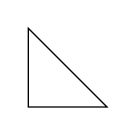
\begin{tikzpicture}
    \draw (1,0) -- (0,0) -- (0,1) -- cycle;
\end{tikzpicture}

\paragraph{Move-to operation}
\begin{Verbatim}[fontsize=\scriptsize]
    \draw (0,0) -- (2,0) (0,1) -- (2,1);
\end{Verbatim}
\begin{tikzpicture}
    \draw (0,0) -- (2,0) (0,1) -- (2,1);
\end{tikzpicture}

\paragraph{Connect points by first horizontal then vertical}
\begin{Verbatim}[fontsize=\scriptsize]
    \draw (0,0) -| (1,1);
\end{Verbatim}
\begin{tikzpicture}
    \draw (0,0) -| (1,1);
\end{tikzpicture}

\paragraph{Connect points by first vertical then horizontal}
\begin{Verbatim}[fontsize=\scriptsize]
    \draw (0,0) |- (1,1);
\end{Verbatim}
\begin{tikzpicture}
    \draw (0,0) |- (1,1);
\end{tikzpicture}

\subsubsection{Drawing curved paths}
\paragraph{Bezier curve using \texttt{controls} command}
\begin{Verbatim}[fontsize=\scriptsize]
    \draw (0,0) .. controls (1,1) .. (4,0)
    (5,0) .. controls (6,0) and (6,1) .. (5,2);
\end{Verbatim}
\begin{tikzpicture}
    \draw (0,0) .. controls (1,1) .. (4,0)
    (5,0) .. controls (6,0) and (6,1) .. (5,2);
\end{tikzpicture}

\paragraph{User-defined paths using the \texttt{to} operation}
\begin{Verbatim}[fontsize=\scriptsize]
    \draw (0,0) to (3,2);
    \draw (0,0) to[out=90,in=180] (3,2);
    \draw (0,0) to[bend right] (3,2);
\end{Verbatim}
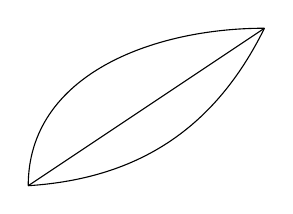
\begin{tikzpicture}
    \draw (0,0) to (3,2);
    \draw (0,0) to[out=90,in=180] (3,2);
    \draw (0,0) to[bend right] (3,2);
\end{tikzpicture}

\subsubsection{Special curves}
% \paragraph{}
% \begin{Verbatim}[fontsize=\scriptsize]

% \end{Verbatim}
% \begin{tikzpicture}

% \end{tikzpicture}

\paragraph{Arrow tips to lines}
\begin{Verbatim}[fontsize=\scriptsize]
    \draw [->] (0,0) -- (30:20pt);
    \draw [<->] (1,0) arc (180:30:10pt);
    \draw [<<->] (2,0) -- ++(0.5,10pt) -- ++(0.5,-10pt) -- ++(0.5,10pt);
\end{Verbatim}
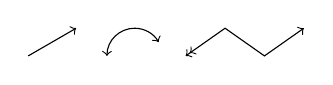
\begin{tikzpicture}
    \draw [->] (0,0) -- (30:20pt);
    \draw [<->] (1,0) arc (180:30:10pt);
    \draw [<<->] (2,0) -- ++(0.5,10pt) -- ++(0.5,-10pt) -- ++(0.5,10pt);
\end{tikzpicture}

\paragraph{Loop using \texttt{foreach} command}
\begin{Verbatim}[fontsize=\scriptsize]
    \foreach \x in {0,...,9}
    \draw (\x,0) circle (0.4);
\end{Verbatim}
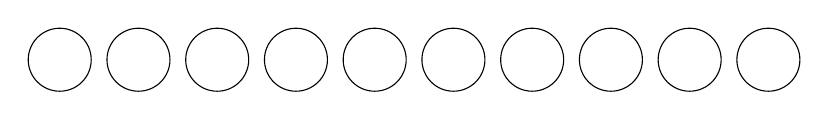
\begin{tikzpicture}
    \foreach \x in {0,...,9}
    \draw (\x,0) circle (0.4);
\end{tikzpicture}

\subsubsection{Nodes}
\paragraph{Draw text along path with node command}
\begin{Verbatim}[fontsize=\scriptsize]
    \draw[dotted]
    (0,0) node {1st node}
    -- (1,1) node {2nd node}
    -- (0,2) node {3rd node}
    -- cycle;
\end{Verbatim}
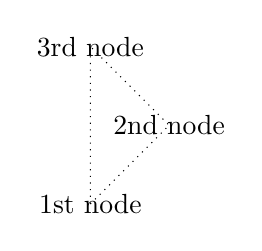
\begin{tikzpicture}
    \draw[dotted]
    (0,0) node {1st node}
    -- (1,1) node {2nd node}
    -- (0,2) node {3rd node}
    -- cycle;
\end{tikzpicture}

\paragraph{Connect nodes using nodes' labels as coordinates (Option 1)}
\begin{Verbatim}[fontsize=\scriptsize]
    \path (0,0) node(x) {}
    (3,1) node(y) {};
    \draw (x) -- (y);
\end{Verbatim}
\begin{tikzpicture}
    \path (0,0) node(x) {}
    (3,1) node(y) {};
    \draw (x) -- (y);
\end{tikzpicture}

\paragraph{Connect nodes using nodes' labels as coordinates (Option 2)}
\begin{Verbatim}[fontsize=\scriptsize]
    \coordinate (x) at (0,0);
    \coordinate (y) at (3,1);
    \draw (x) -- (y);
\end{Verbatim}
\begin{tikzpicture}
    \coordinate (x) at (0,0);
    \coordinate (y) at (3,1);
    \draw (x) -- (y);
\end{tikzpicture}

\paragraph{Multi-line text inside a node}
\begin{Verbatim}[fontsize=\scriptsize]
    \filldraw
    (0,0) circle (2pt) node[align=left,   below] {test 1\\is aligned left} --
    (4,0) circle (2pt) node[align=center, below] {test 2\\is centered}     --
    (8,0) circle (2pt) node[align=right,  below] {test 3\\is right aligned};
\end{Verbatim}
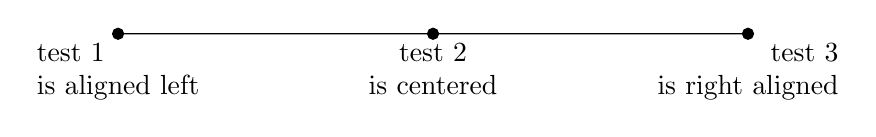
\begin{tikzpicture}
    \filldraw
    (0,0) circle (2pt) node[align=left,   below] {test 1\\is aligned left} --
    (4,0) circle (2pt) node[align=center, below] {test 2\\is centered}     --
    (8,0) circle (2pt) node[align=right,  below] {test 3\\is right aligned};
\end{tikzpicture}

% \paragraph{}
% \begin{Verbatim}[fontsize=\scriptsize]

% \end{Verbatim} 
% \begin{tikzpicture}

% \end{tikzpicture}

\paragraph{For inline}
\begin{Verbatim}[fontsize=\scriptsize]
    \tikz[]{\draw[red, dashed, very thick, rotate=30] (1,0) -- (0,0) -- (0,1);}
\end{Verbatim}
\tikz[]{\draw[red, dashed, very thick, rotate=30] (1,0) -- (0,0) -- (0,1);}

\paragraph{Unit circle on graph}
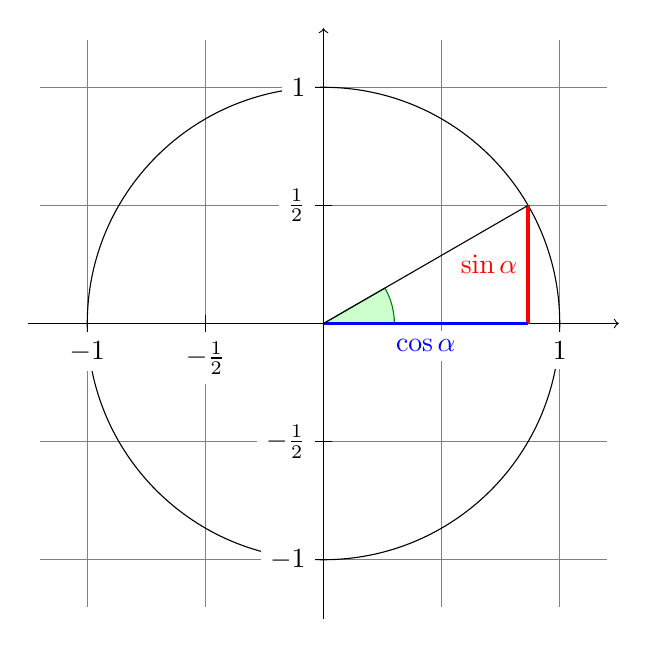
\begin{tikzpicture}[scale=3]
    \draw[step=.5cm, gray, very thin] (-1.2,-1.2) grid (1.2,1.2);
    \filldraw[fill=green!20,draw=green!50!black] (0,0) -- (3mm,0mm) arc (0:30:3mm) -- cycle;
    \draw[->] (-1.25,0) -- (1.25,0) coordinate (x axis);
    \draw[->] (0,-1.25) -- (0,1.25) coordinate (y axis);
    \draw (0,0) circle (1cm);
    \draw[very thick,red] (30:1cm) -- node[left,fill=white] {$\sin \alpha$} (30:1cm |- x axis);
    \draw[very thick,blue] (30:1cm |- x axis) -- node[below=2pt,fill=white] {$\cos \alpha$} (0,0);
    \draw (0,0) -- (30:1cm);
    \foreach \x/\xtext in {-1, -0.5/-\frac{1}{2}, 1}
    \draw (\x cm,1pt) -- (\x cm,-1pt) node[anchor=north,fill=white] {$\xtext$};
    \foreach \y/\ytext in {-1, -0.5/-\frac{1}{2}, 0.5/\frac{1}{2}, 1}
    \draw (1pt,\y cm) -- (-1pt,\y cm) node[anchor=east,fill=white] {$\ytext$};
\end{tikzpicture}

\paragraph{Functions}
\begin{Verbatim}[fontsize=\scriptsize]
    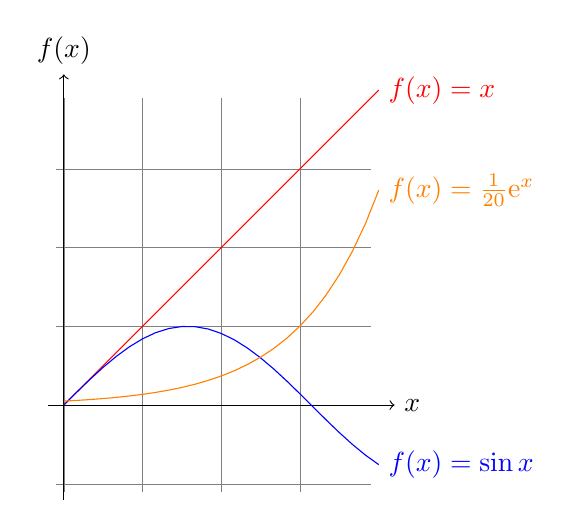
\begin{tikzpicture}[domain=0:4]
        \draw[very thin,color=gray] (-0.1,-1.1) grid (3.9,3.9);
        \draw[->] (-0.2,0) -- (4.2,0) node[right] {$x$};
        \draw[->] (0,-1.2) -- (0,4.2) node[above] {$f(x)$};
        \draw[color=red]    plot (\x,\x)             node[right] {$f(x) =x$};
        \draw[color=blue]   plot (\x,{sin(\x r)})    node[right] {$f(x) = \sin x$};
        \draw[color=orange] plot (\x,{0.05*exp(\x)}) node[right] {$f(x) = \frac{1}{20} \mathrm e^x$};
    \end{tikzpicture}
\end{Verbatim}



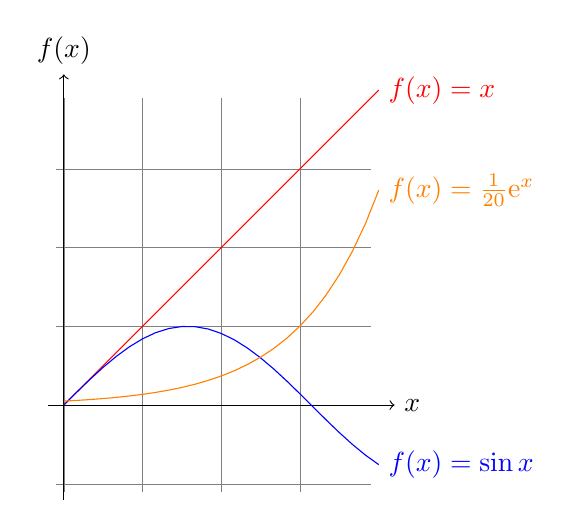
\begin{tikzpicture}[domain=0:4]
    \draw[very thin,color=gray] (-0.1,-1.1) grid (3.9,3.9);
    \draw[->] (-0.2,0) -- (4.2,0) node[right] {$x$};
    \draw[->] (0,-1.2) -- (0,4.2) node[above] {$f(x)$};
    \draw[color=red]    plot (\x,\x)             node[right] {$f(x) =x$};
    \draw[color=blue]   plot (\x,{sin(\x r)})    node[right] {$f(x) = \sin x$};
    \draw[color=orange] plot (\x,{0.05*exp(\x)}) node[right] {$f(x) = \frac{1}{20} \mathrm e^x$};
\end{tikzpicture}

\paragraph{Shape with rounded corners}
\begin{Verbatim}[fontsize=\scriptsize]
    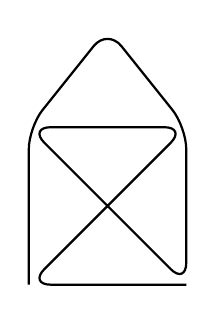
\begin{tikzpicture}
        \draw[thick,rounded corners=8pt] (0,0) -- (0,2) -- (1,3.25)
        -- (2,2) -- (2,0) -- (0,2) -- (2,2) -- (0,0) -- (2,0);
    \end{tikzpicture}
\end{Verbatim}
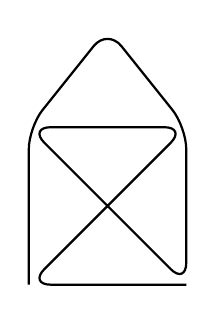
\begin{tikzpicture}
    \draw[thick,rounded corners=8pt] (0,0) -- (0,2) -- (1,3.25)
    -- (2,2) -- (2,0) -- (0,2) -- (2,2) -- (0,0) -- (2,0);
\end{tikzpicture}

\subsection{Letters}
TODO: \href{https://en.wikibooks.org/wiki/LaTeX/Letters}{Letters}
\subsection{Source code}
TODO: \href{https://en.wikibooks.org/wiki/LaTeX/Source_Code_Listings}{Source code listings}

\subsection{Comments on equations}
\subsubsection{Comment on parts}
\[
    z = \overbrace{
        \underbrace{x}_\text{real} + i
        \underbrace{y}_\text{imaginary}
    }^\text{complex number}
\]

\subsubsection{Comments longer than formula}
\[
    y = a + f(\underbrace{b x}_{
    \ge 0 \text{ by assumption}})
    = a + f(\underbrace{b x}_{
    \mathclap{\ge 0 \text{ by assumption}}})
\]





% \noindent\rule{8cm}{0.4pt}

% Below is a Line spanning the entire width of the page

% \noindent\makebox[\linewidth]{\rule{\paperwidth}{0.4pt}}

% Below is a 2cm long line

% \noindent\rule{2cm}{0.4pt}

% Below is a 4cm long line

% \noindent\rule{4cm}{0.4pt}

% Below is a 8cm long line

% \noindent\rule{8cm}{0.4pt}

% \begin{align*}
%     \left\lfloor\dfrac{n}{d}\right\rfloor &= \frac{n + d - 1}{d} \\
%     \Bigl\lfloor\dfrac{n}{d}\Bigr\rfloor\qquad &= \frac{n + d - 1}{d} \\
%     \floor*{\frac{n}{d}} &= \frac{n + d - 1}{d}
% \end{align*}

% \[
% \floor[\Big]{\frac{1}{2}}
% \qquad
% \floor[\bigg]{\frac{1}{2}}
% \qquad
% \floor*{\frac{1}{2}}  % autosize vertical dim. of brackets
% \]


\end{document}

